\begin{figure}[t]
\centering
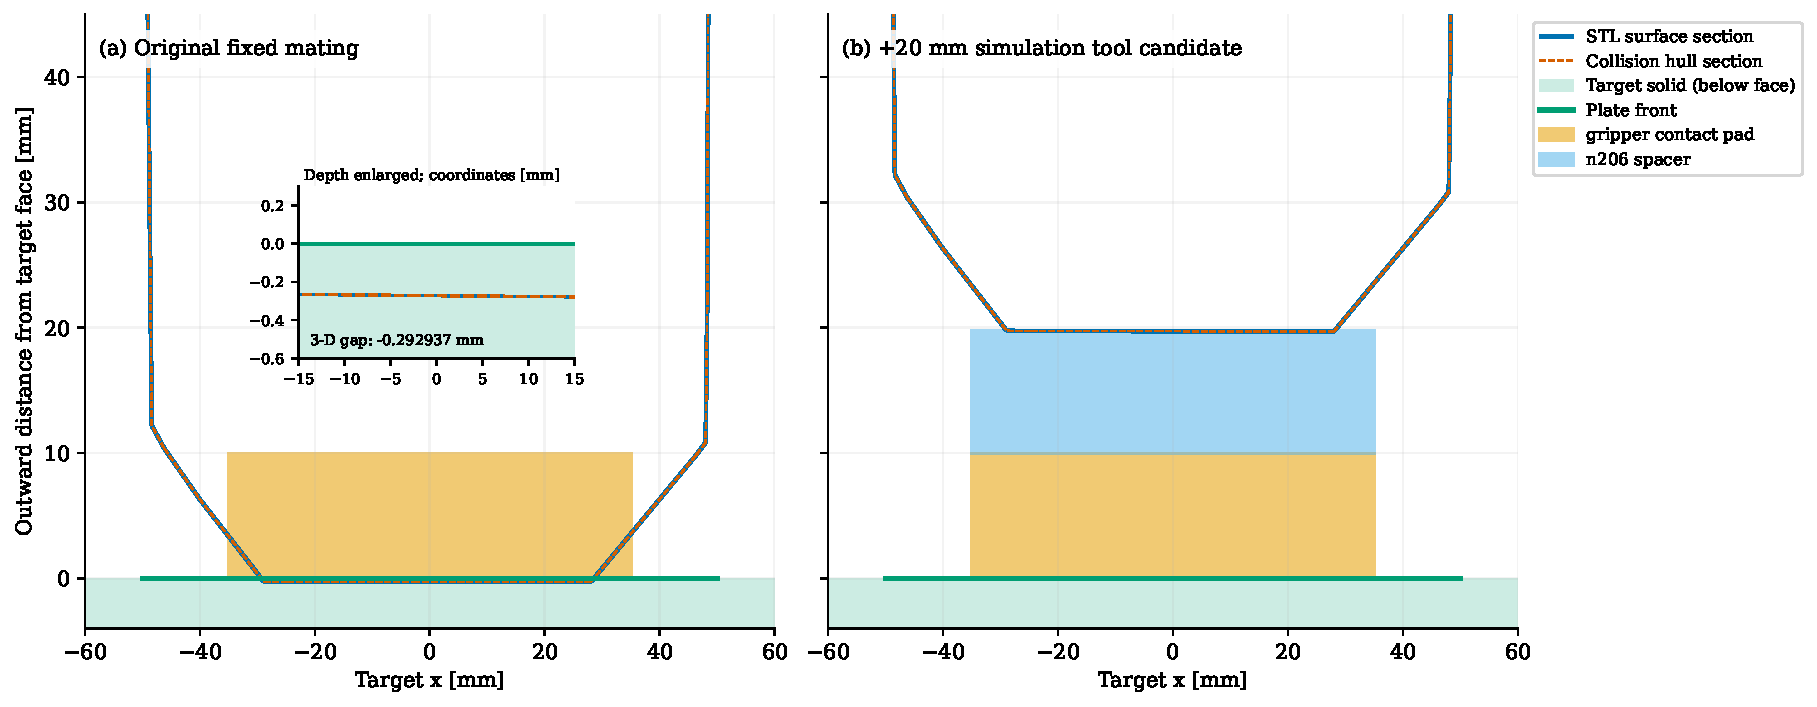
\includegraphics[width=\linewidth]{terminal_sections.pdf}
\caption{Ideal mating in the target frame; STL and convex-hull sections at target z=0. Tool solids projected into that plane (interface tilt is under 0.002 deg). Original global 3-D link7 distance -0.292936604 mm; 20 mm candidate gives about +19.707063 mm. These query distances are not inferred from the 2-D section. Inset magnifies the depth coordinate. New 9.8 mm spacer and 10 mm pad use a rigid circular-seat simulation assumption, not approved hardware. Old/new main panels use identical axes and original STL scale.}
\end{figure}

\begin{figure}[t]
\centering
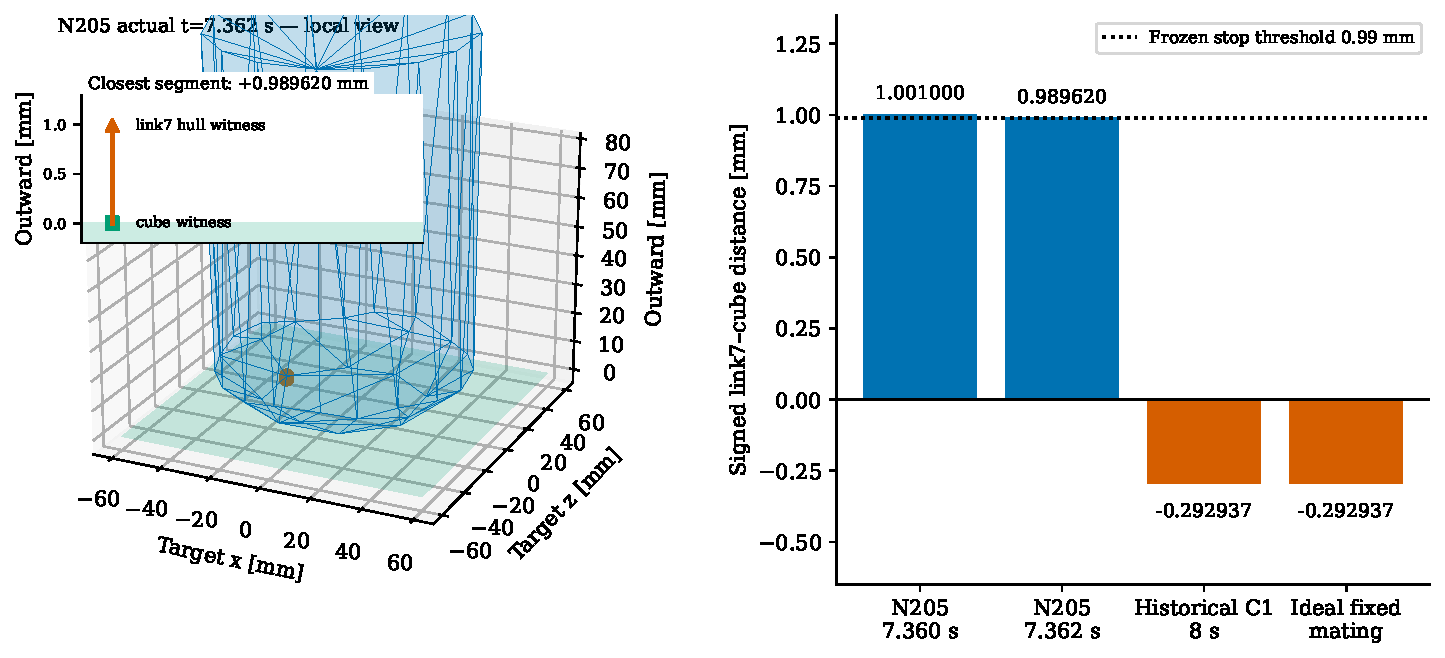
\includegraphics[width=\linewidth]{failure_witness.pdf}
\caption{Left: N205 actual 7.362 s saved state; supplied STL surface triangles, target face and geometrically labelled closest points. Gap is positive +0.989619610 mm; no collision asserted. Right: actual N205 samples and separate historical/ideal static queries. Historical and ideal negative distances also have 29 triangle/box crossing witnesses; this is not solely convex-hull filling. Geometry is supplied collision STL, not certified CAD.}
\end{figure}

\begin{figure}[t]
\centering
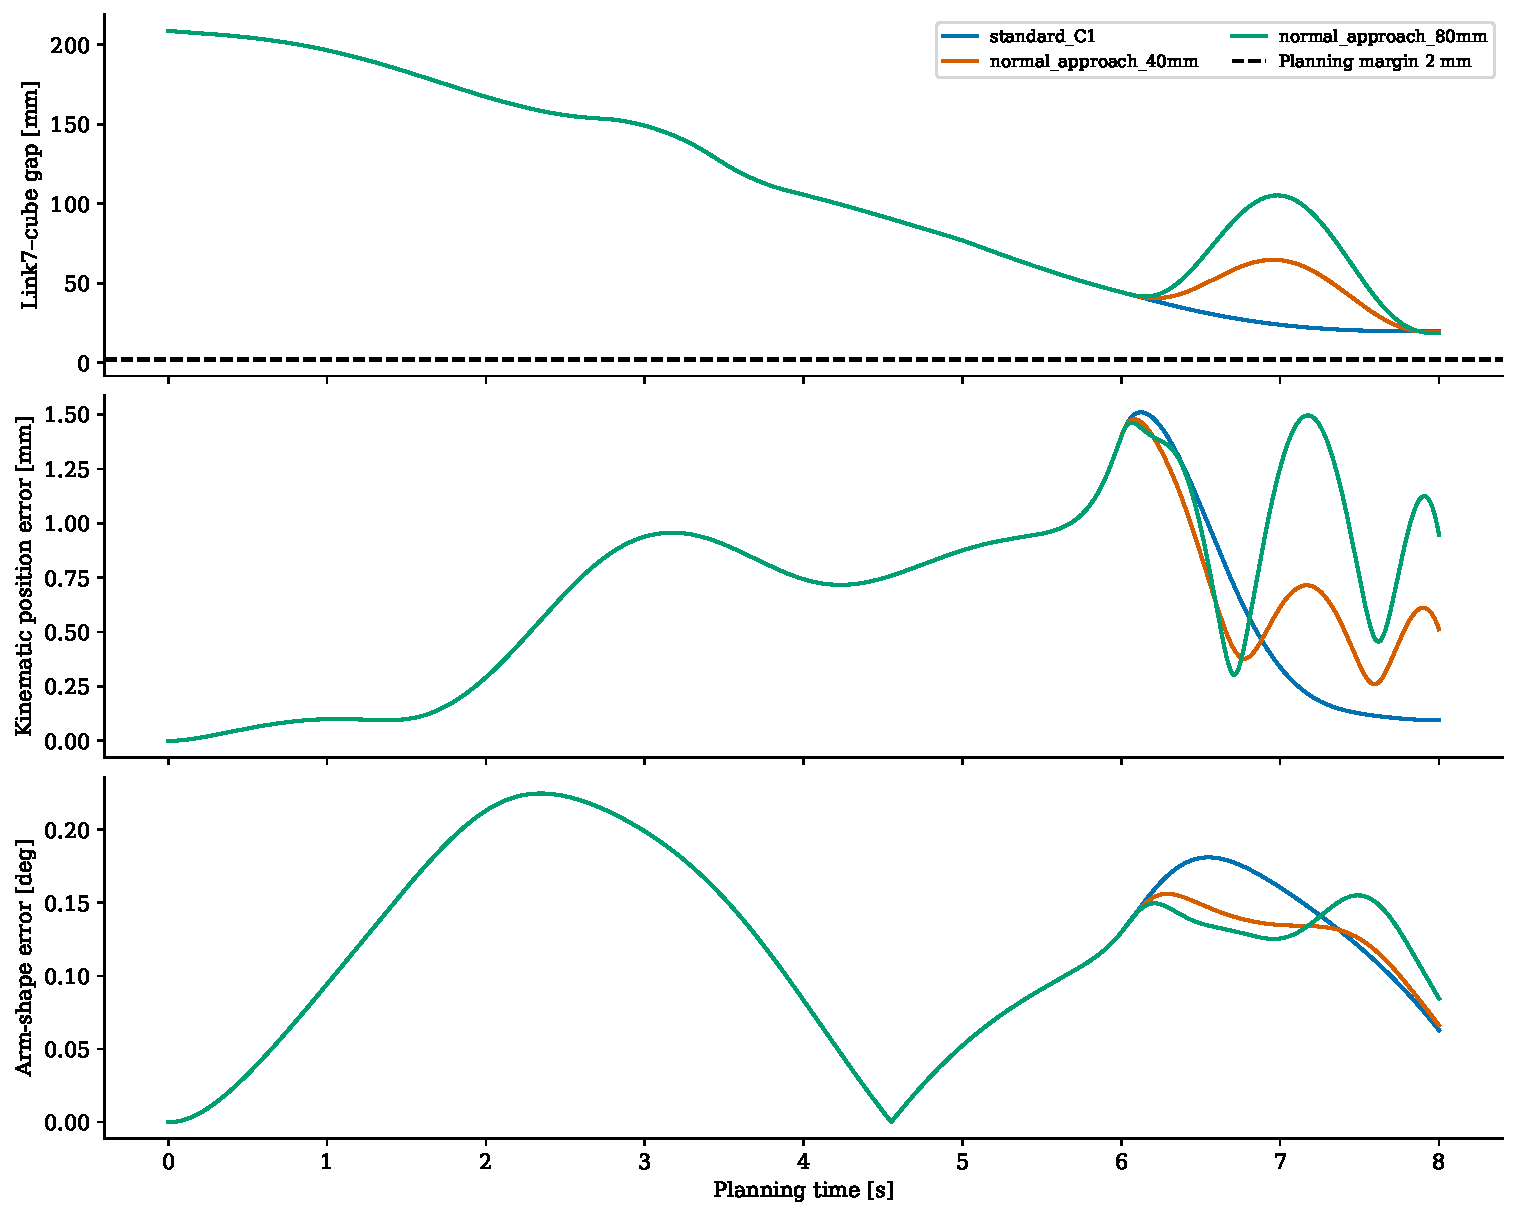
\includegraphics[width=\linewidth]{planning_screening.pdf}
\caption{Three frozen references, all sampled over 0–8 s with added target/tool pairs in hard distance constraints. These are kinematic planning integrations, not true closed-loop dynamics. Same-path adaptive interval checks use 0.5 ms for standard C1 and 0.25 ms for other candidates near pad contact; no arbitrary perturbation guarantee. Standard C1 selected without reading postgrasp results.}
\end{figure}

\begin{figure}[t]
\centering
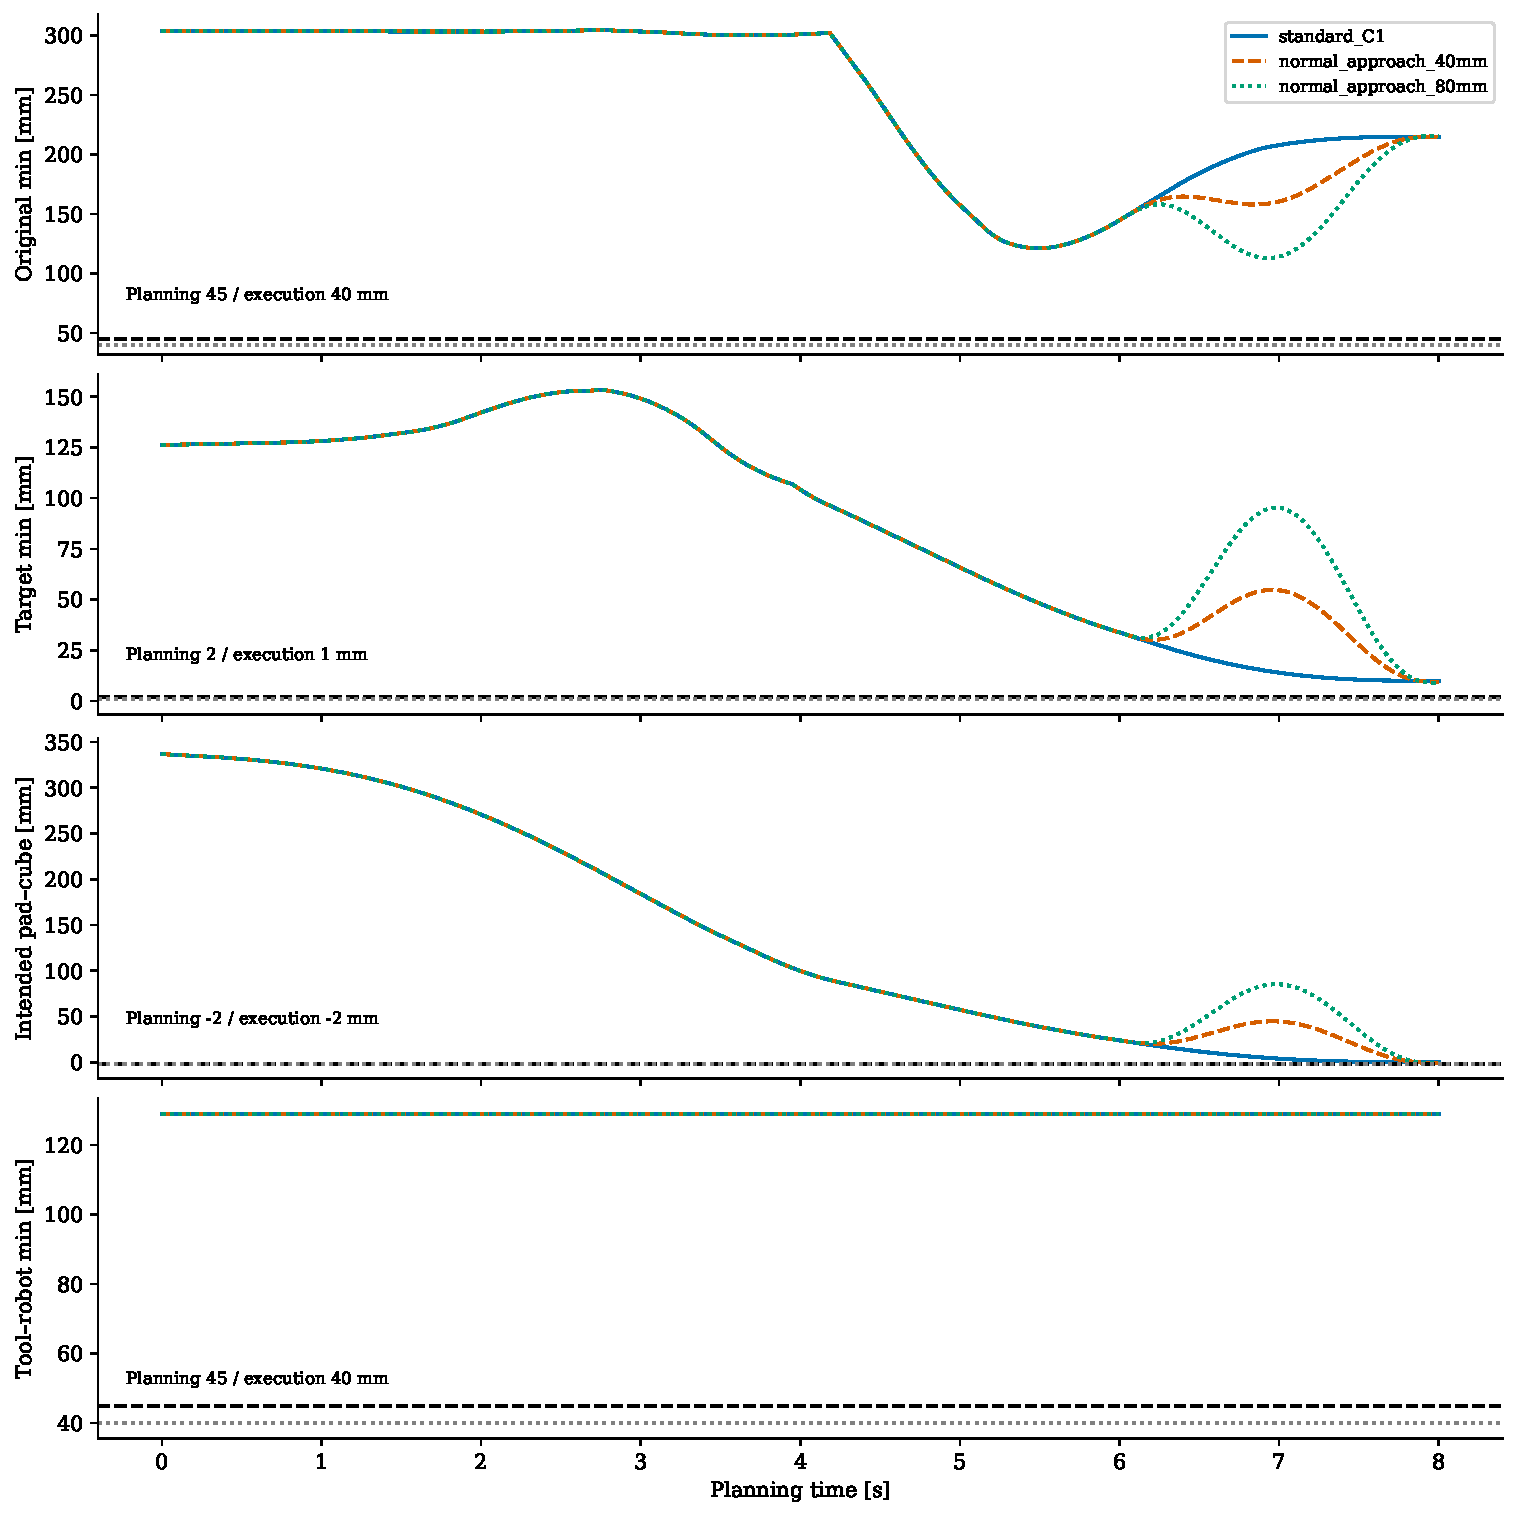
\includegraphics[width=\linewidth]{planning_pair_classes.pdf}
\caption{Pointwise minimum within each pair class for all frozen kinematic planning candidates: original 24 pairs, unintended target pairs, intended pad–cube and added tool–robot/obstacle pairs. No real closed-loop dynamics shown. Dashed black lines: planning gates; dotted grey: unchanged execution gates before numeric tolerance. Candidate curves overlap before 6 s. Per-pair conservative interpolation bounds and adaptive checks are in trajectory\_screening.json. Stated tool simulation assumption only, not hardware verification.}
\end{figure}

\begin{figure}[t]
\centering
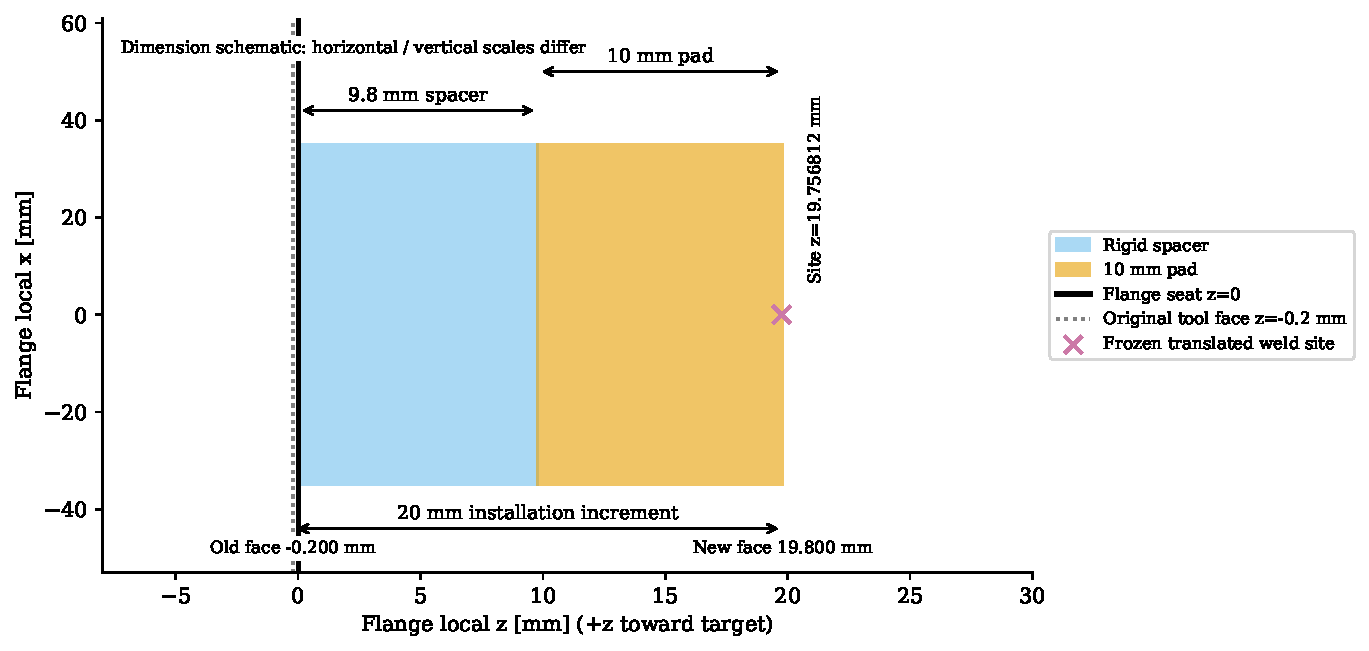
\includegraphics[width=\linewidth]{tool_dimension_drawing.pdf}
\caption{Simulation dimension drawing in the flange frame. Radius 35 mm; 9.8 mm positive-length spacer contiguous with the 10 mm pad; 20 mm is installation increment, not spacer thickness. Added aluminium-equivalent density 2700 kg/m³, total mass 0.205738 kg, explicit positive inertia. Entire circular rigid seat assumed; no bolt pattern, manufacturing CAD, strength or hardware approval. Target geometry and robot flange/link7 unchanged.}
\end{figure}

\begin{figure}[t]
\centering
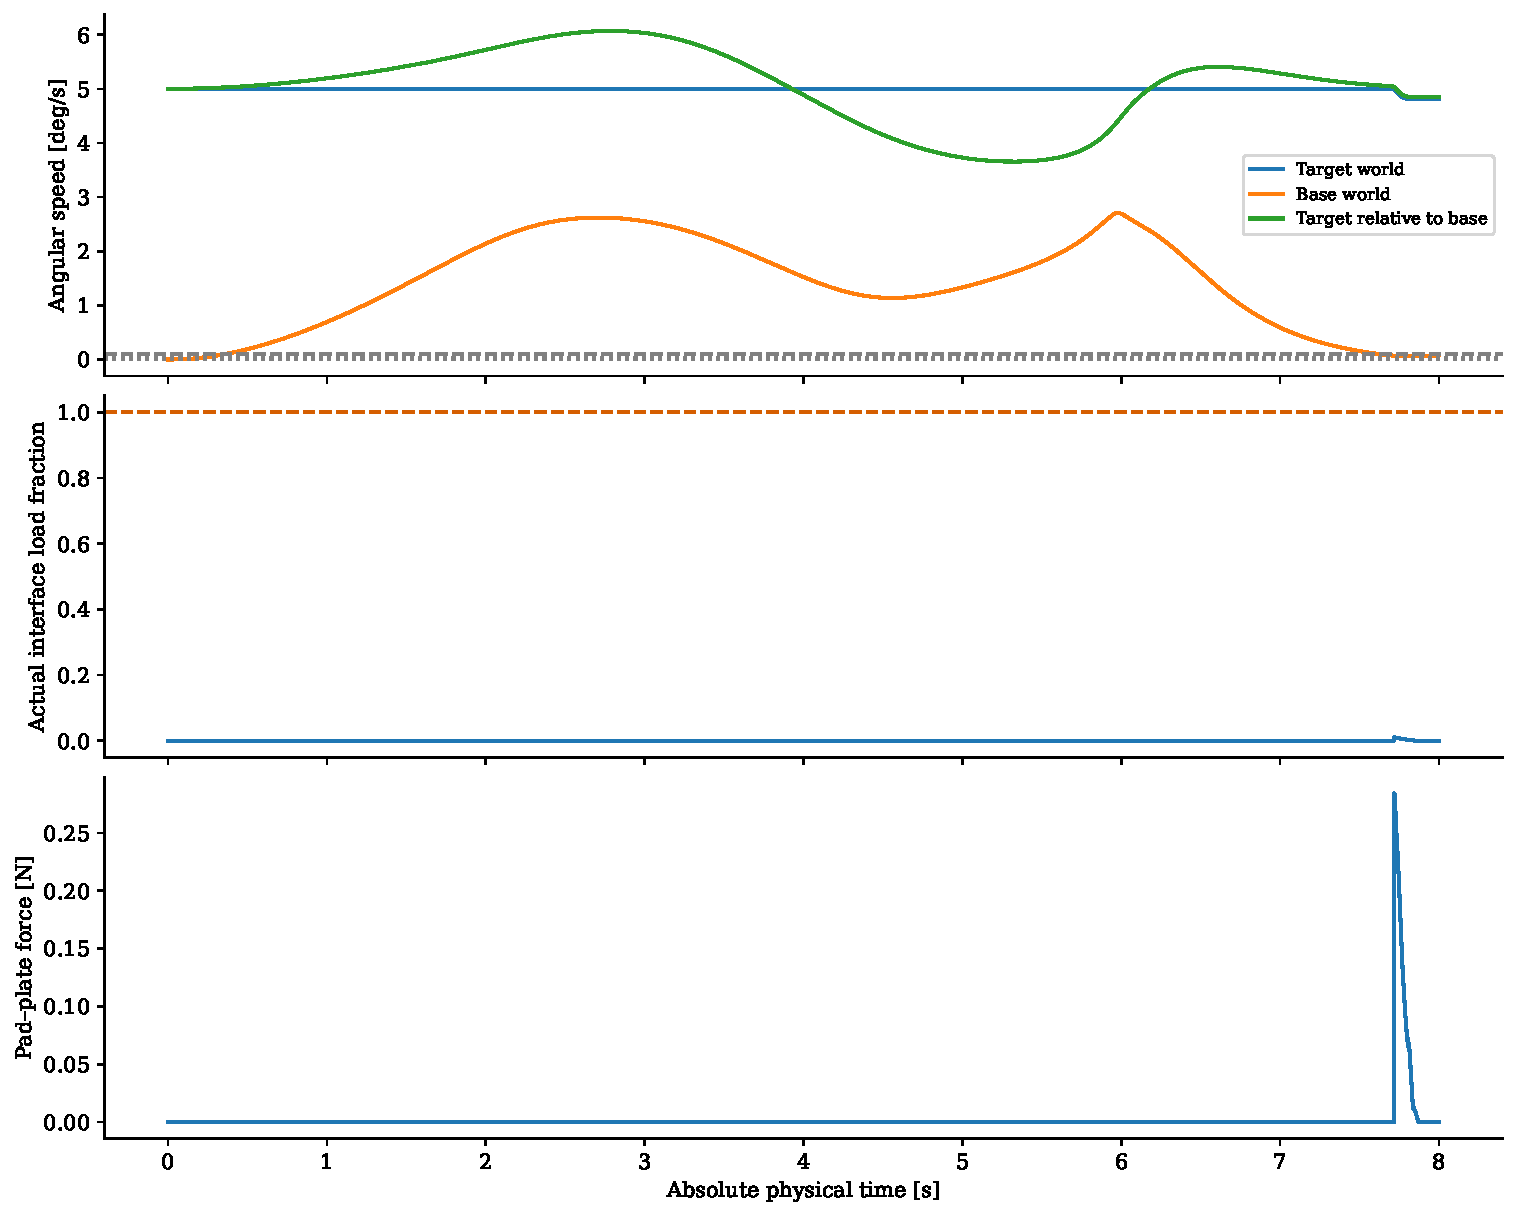
\includegraphics[width=\linewidth]{angular_speed_load_contact.pdf}
\caption{N206 nominal actual continuous dynamics through 8.000 s. [16,18] s NOT EVALUATED. Angular speed gates are fixed at 0.1 and 0.02 deg/s. Load fraction uses the actual physical wrench and original 50 N / 2 Nm envelope; no old postgrasp curves inherited.}
\end{figure}

\begin{figure}[t]
\centering
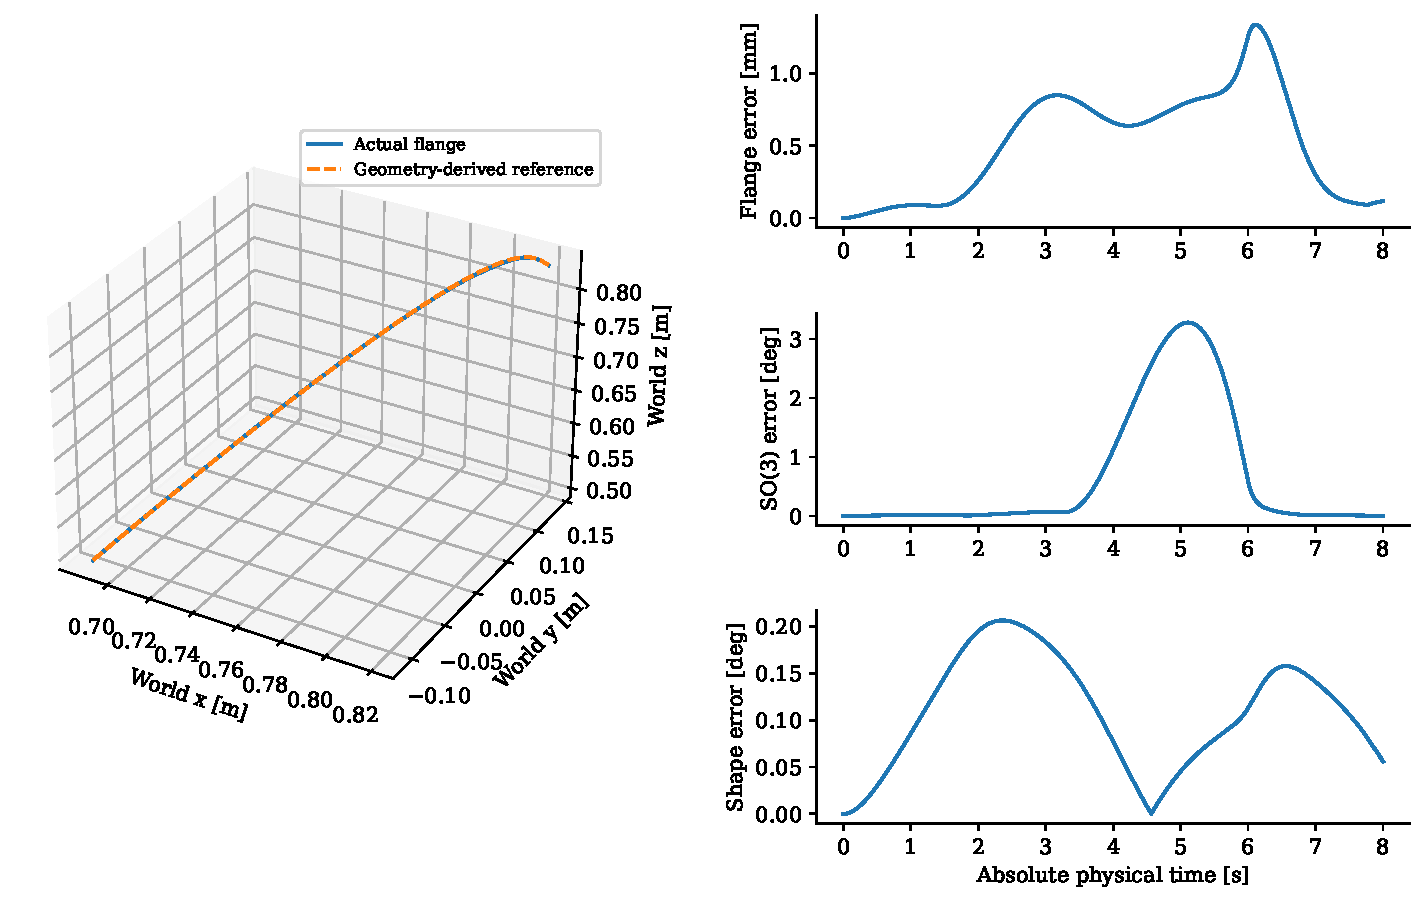
\includegraphics[width=\linewidth]{end_effector_tracking.pdf}
\caption{N206 actual flange path and approach tracking errors from home through min(8,8.000) s. Reference comes from new fixed flange–tool and target–grasp transforms; it does not fit an old actual terminal state. These errors are distinct from postgrasp holding errors.}
\end{figure}

\begin{figure}[t]
\centering
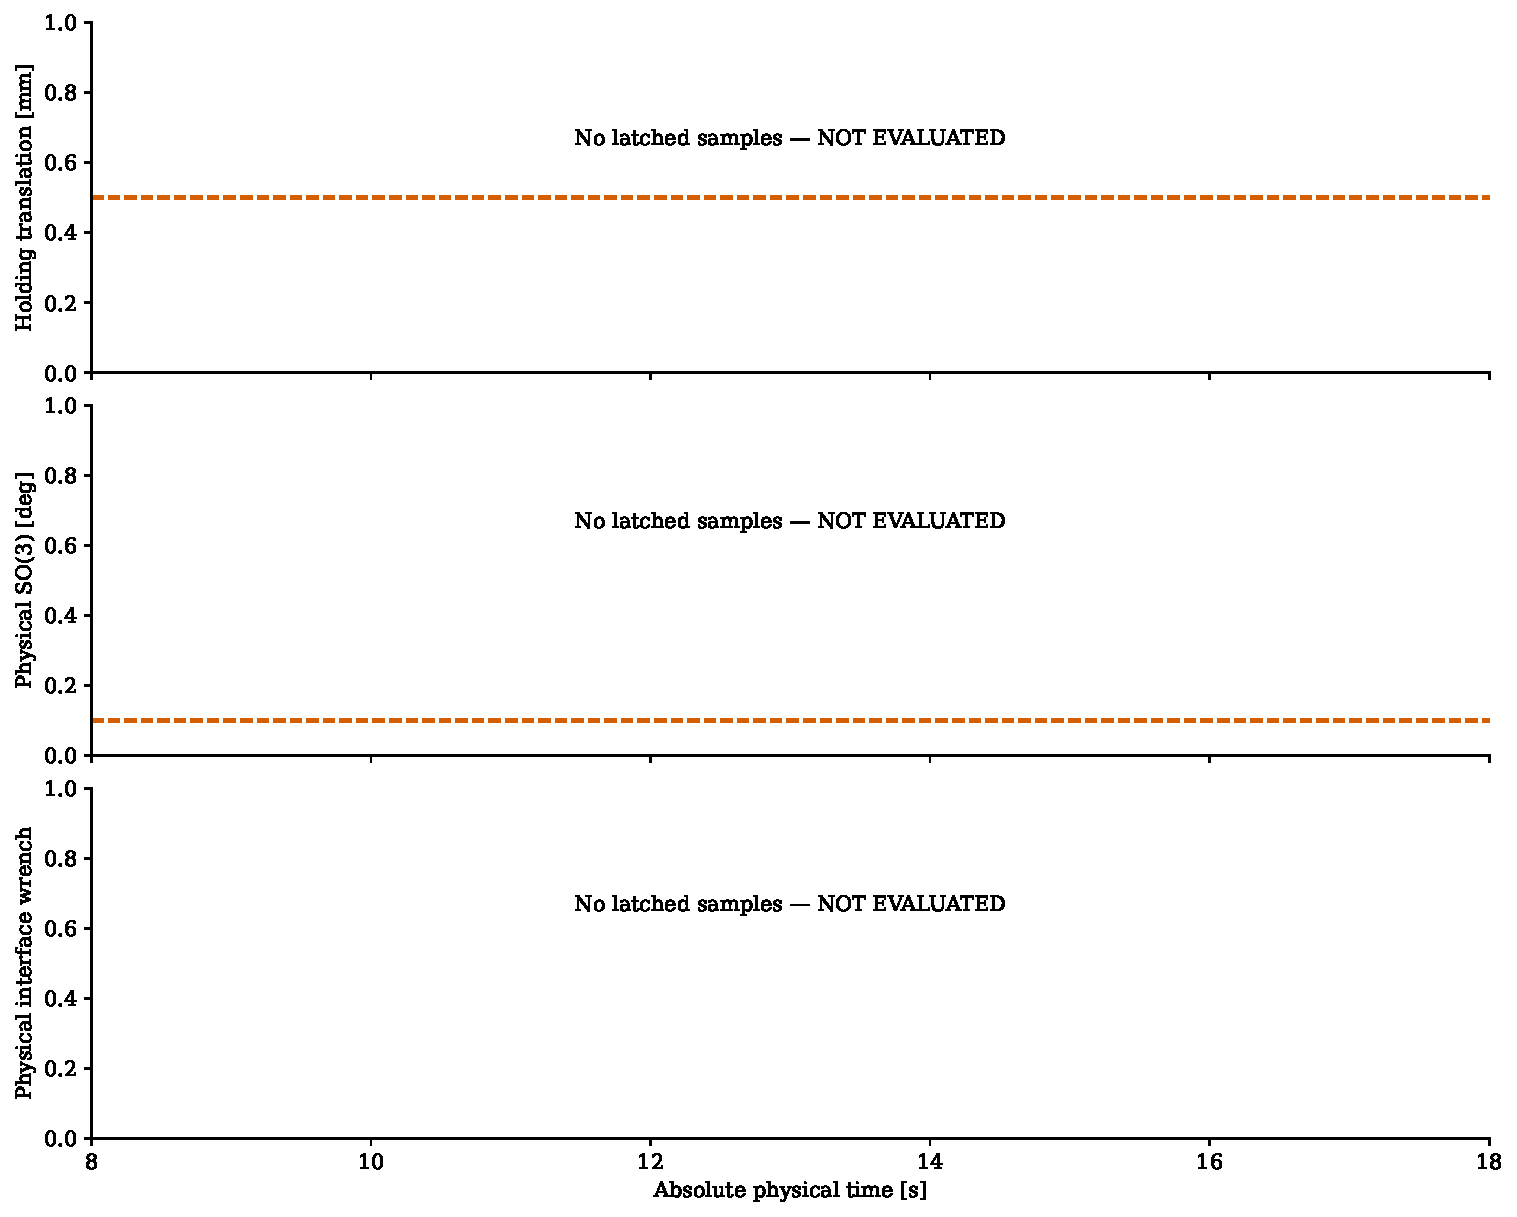
\includegraphics[width=\linewidth]{interface_holding.pdf}
\caption{Only actual latched samples are plotted; nominal ended at 8.000 s. No holding curves fabricated for an unexecuted stage. Original 0.5 mm / 0.1 deg limits and physical wrench reference remain fixed.}
\end{figure}

\begin{figure}[t]
\centering
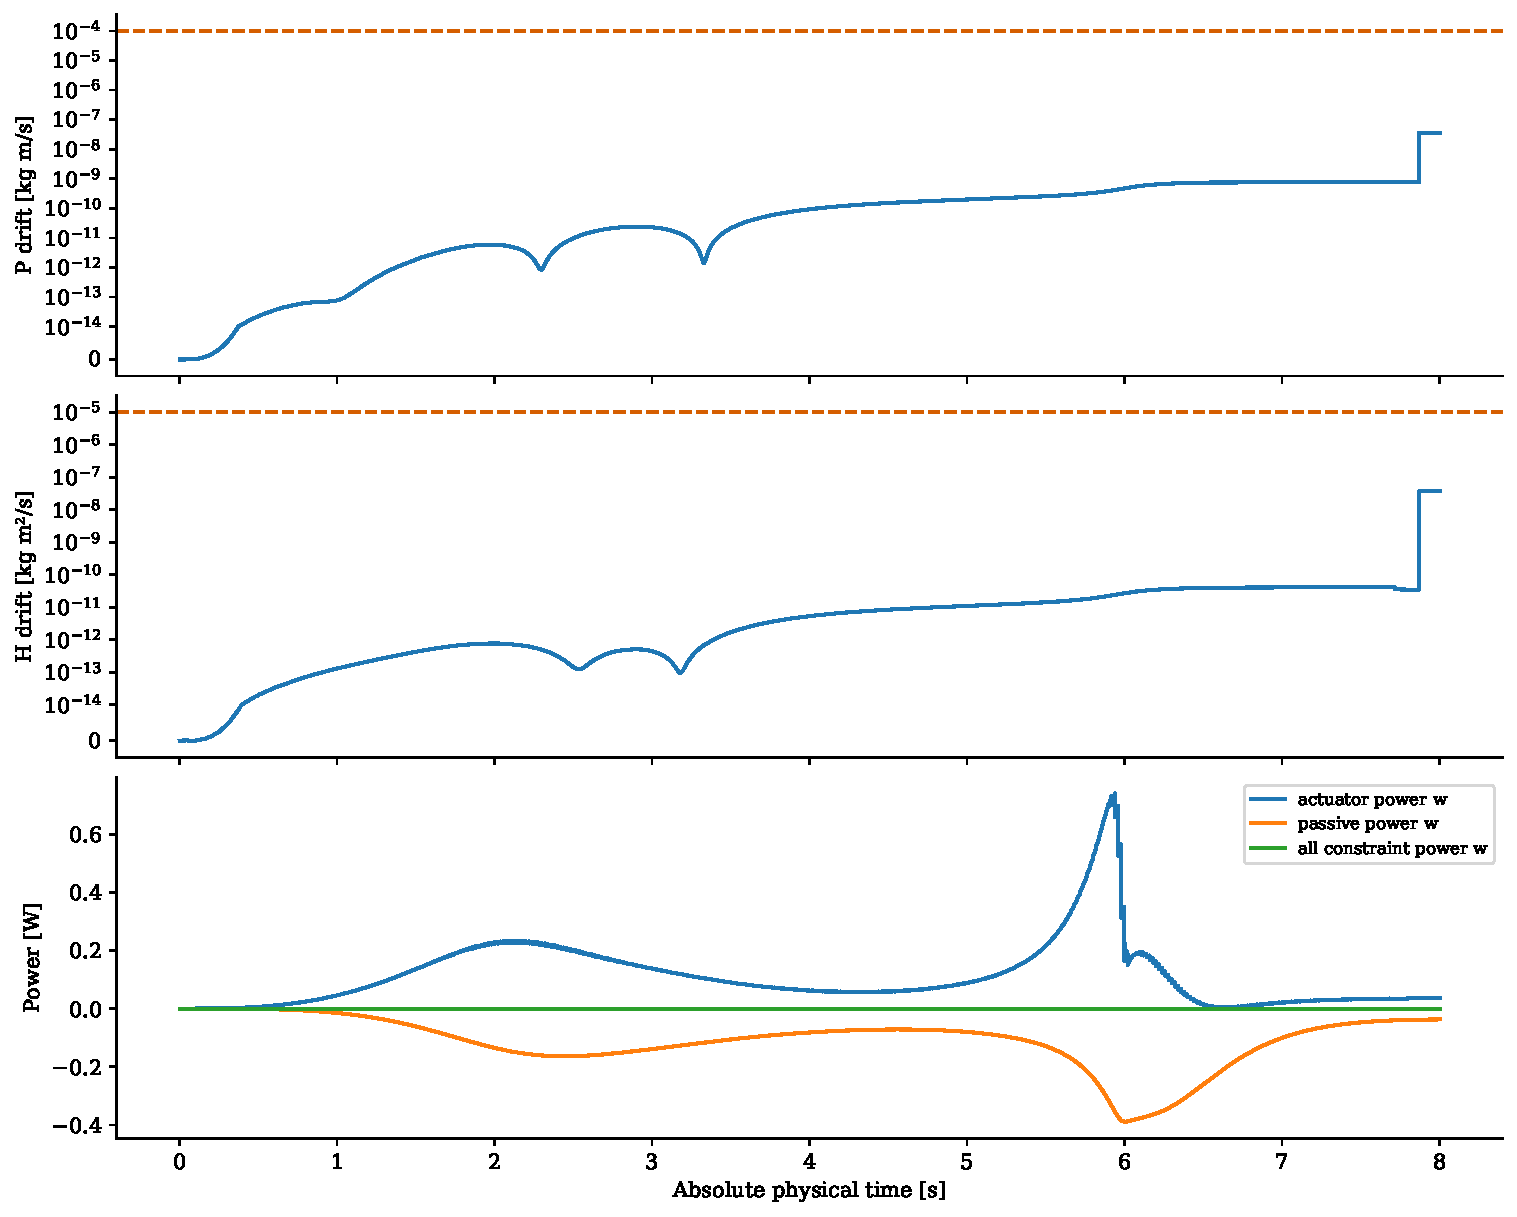
\includegraphics[width=\linewidth]{momentum_power.pdf}
\caption{Whole physical robot + target system, referenced to actual t=0. The kinematically prescribed visualization marker is excluded from COM and locked-inertia accounting without altering the MuJoCo plant. Actuator, passive and constraint powers remain physical quantities.}
\end{figure}

\begin{figure}[t]
\centering
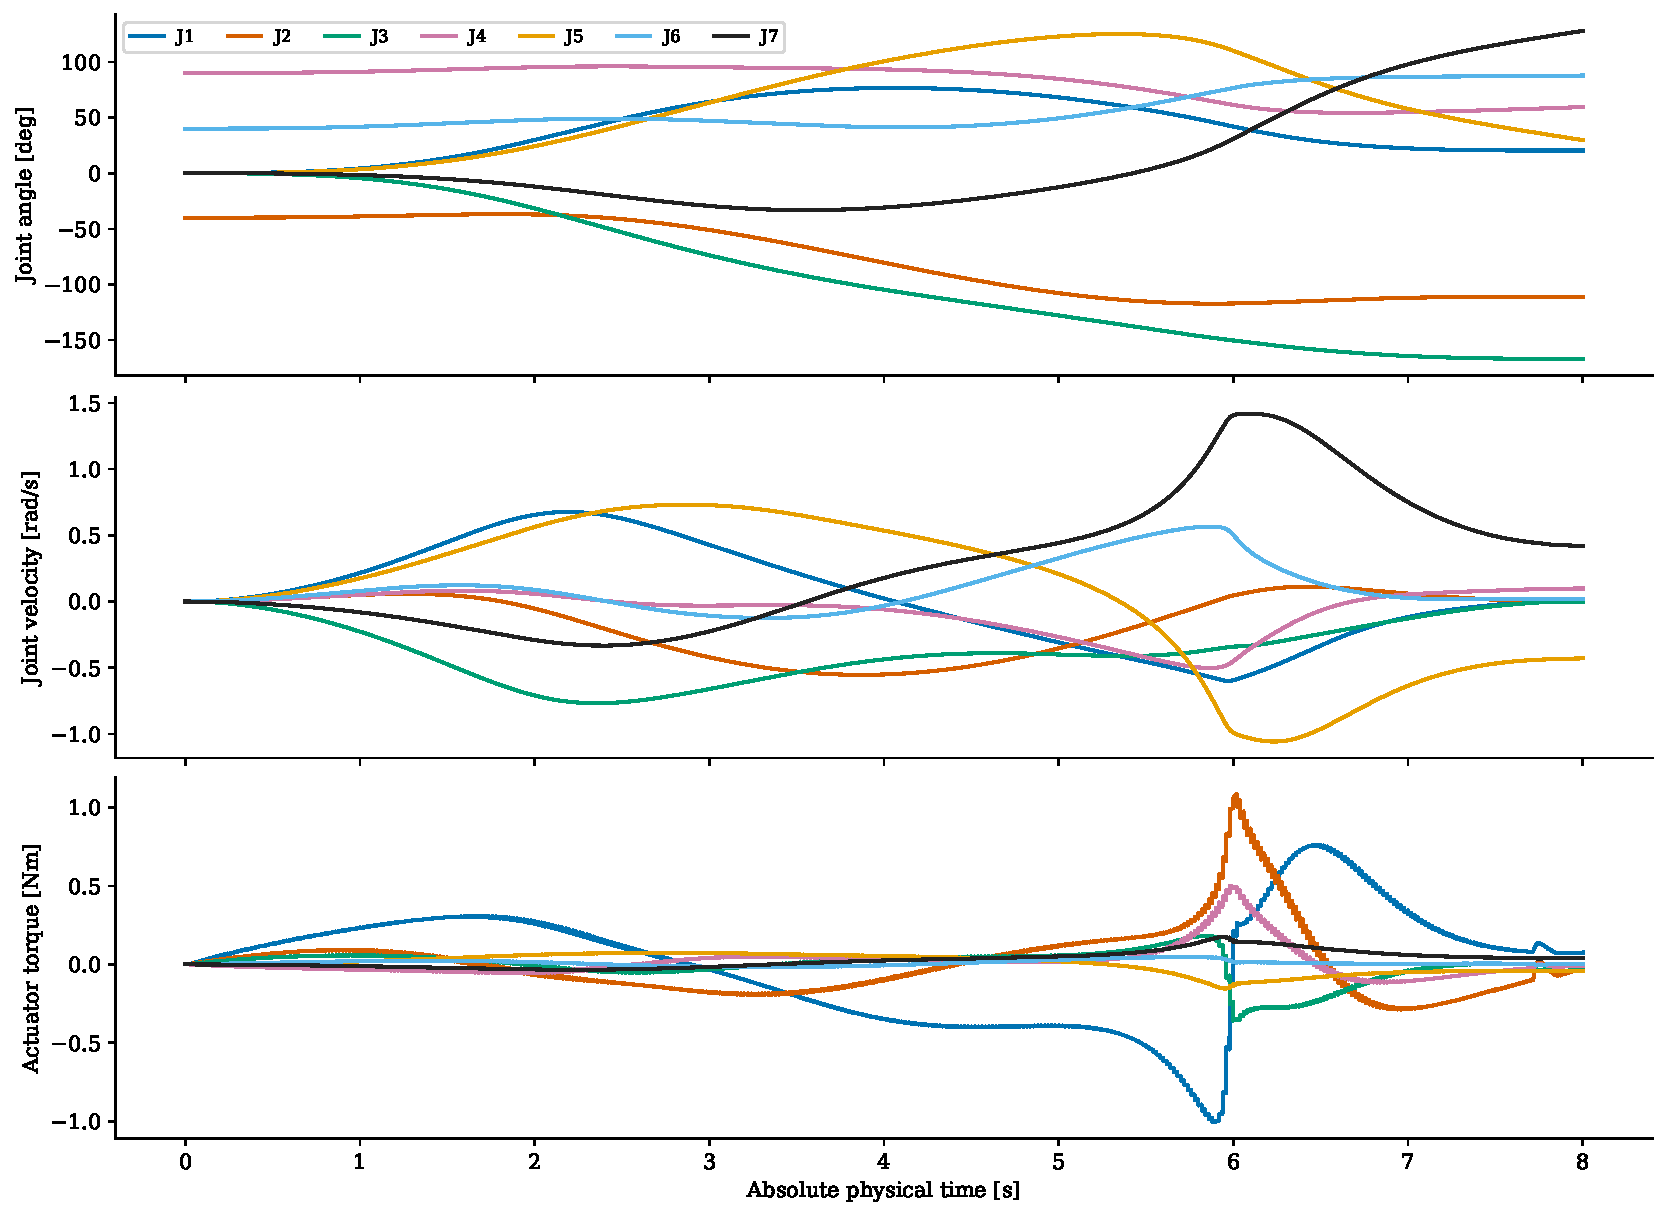
\includegraphics[width=\linewidth]{joints_and_torque.pdf}
\caption{All seven driven joints during N206 actual nominal dynamics. Torque is measured actuator force in joint units; individual original limits are checked numerically in validation, with no retuning.}
\end{figure}

\begin{figure}[t]
\centering
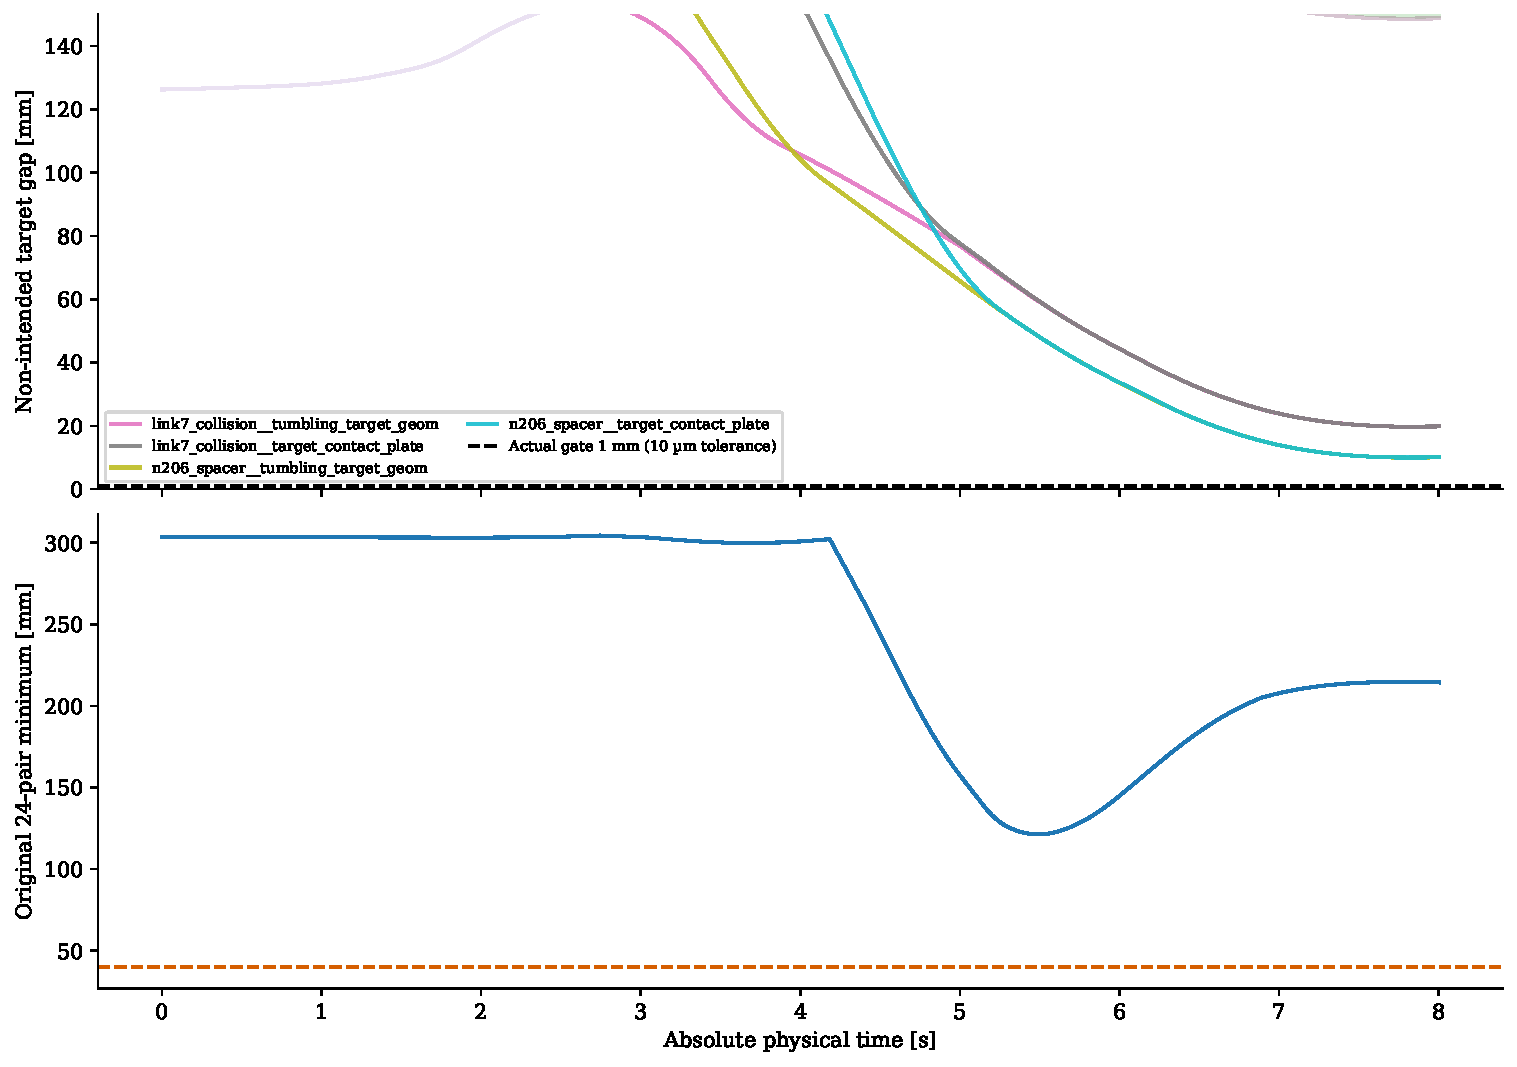
\includegraphics[width=\linewidth]{distance_safety.pdf}
\caption{Actual N206 distances through 8.000 s. Link7 and spacer remain monitored during every phase. Original 24 pairs keep 40 mm execution / 45 mm planning margins; new target pairs use 1 mm execution / 2 mm planning. Pad–cube intended-face exception is recorded separately, never applied to link7 or spacer.}
\end{figure}

\begin{figure}[t]
\centering
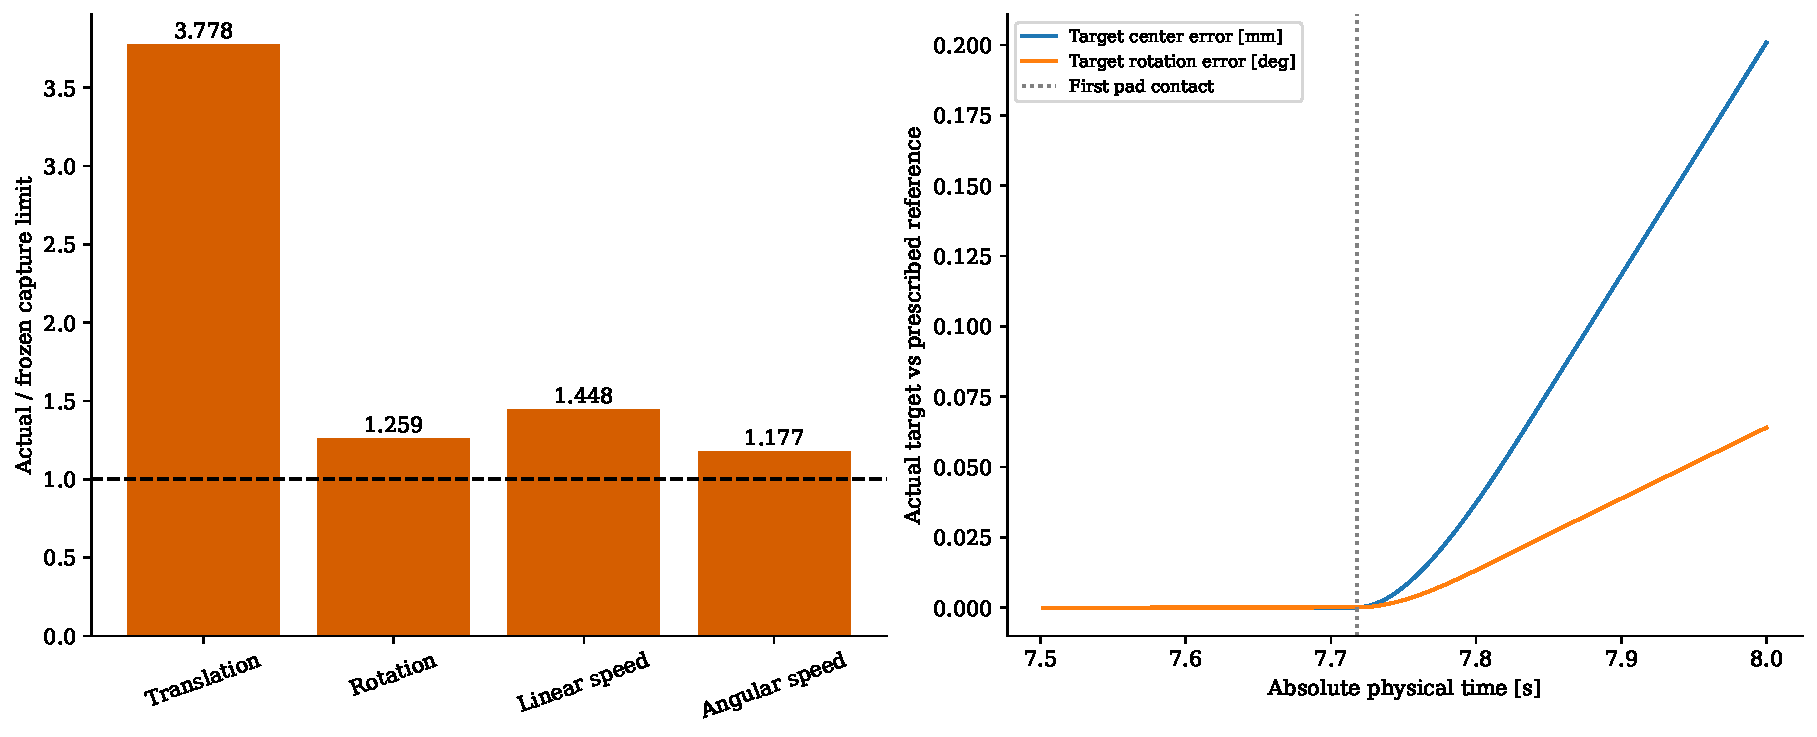
\includegraphics[width=\linewidth]{capture_gate_failure.pdf}
\caption{Actual t=8 capture metrics normalized by unchanged limits: 0.1 mm, 0.05 deg, 1 mm/s, 0.2 deg/s. All four fail and latch remains inactive. Right: real target divergence after first detected intended contact; mixed units explicitly labelled. Temporal sequence is evidence from the one actual trace, not a counterfactual causal experiment. No new reference or controller tuning followed.}
\end{figure}

\begin{figure}[t]
\centering
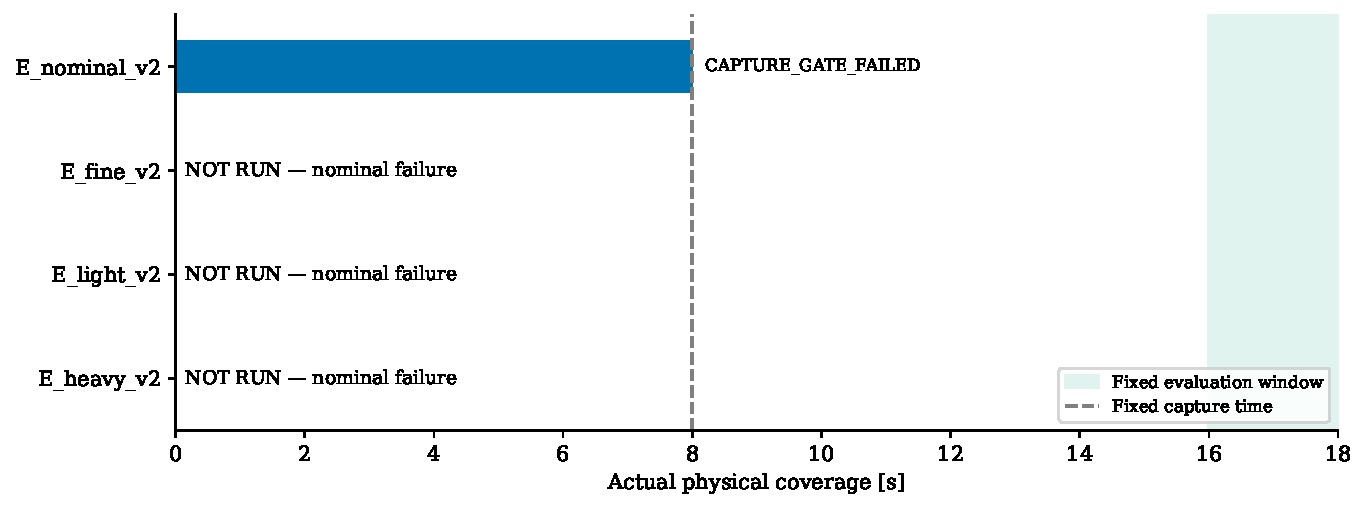
\includegraphics[width=\linewidth]{run_coverage.pdf}
\caption{Only actual integrated duration is filled. Unexecuted fine/light/heavy cases are labelled NOT RUN and are not represented as zero-valued measurements. Capture time stays 8 s and final evaluation window stays [16,18] s, even when the nominal trajectory stops.}
\end{figure}